


\subsection{Simulación de las trayectorias}

% B- Módulo de generación de trayectorias
% - Objetivo del módulo		
La modelización de las trayectorias nos permite conseguir una primera visión del comportamiento de nuestro algoritmo antes de la pruebas experimentales. Los modelos de movimiento del objetivo toman importancia, ya que de ello dependerá la similitud con la realidad.
% - Modelización
%       - trayectoria

En navindoor, las trayectorias son creadas a partir de una sucesión de puntos dentro de una planimetría previamente definida. Estos puntos definen los tramos por donde se transladará el objetivo. Gracias a la información obtenida de la planimetría, se puede generar distintos modelos para cada tramo, tiendo en cuenta sus características. 
%       - velocidad

Un vez definida los puntos por donde pasará el objetivo, a partir de modelos de simulación, se genera una sucesión de puntos más fina que además de contener las cordenadas del punto, contiene el instante en el tiempo cuando esta en éste. De esta forma, las velocidades y aceleraciones pueden ser obtenidas mediante diferenciación.
%       - Ground truths:
%               - trayectoria COM
%               - trayectoria foot-mounted	

Los modelos de generación de la trayectorias estan centrados en la simlulación del pie de un peatón. A partir de ésta se crear otra trayectoria asociada que representa el movimiento del centro de masas, esta es llamada \emph{GroundTruth} de referencia. Estas dos \emph{GroundTruth}s, son indispensable para la definición de la trayectoria. La trayectoria del centro de masas es utilizada par la generación de señales que son medidas en el centro del peatón, mientras que la trayectoria del pie, es utilizada para la generación de señales inerciales. La generación del \emph{GroundTruth} del pie por defecto sigue el modelo de simulación propuesto en el artículo \cite{Zampella2011}, mientras la simulación de cambio de plantas se realiza con un modelo simplificado de velocidad constante.
%       - Diagrama de clases
En la figura \ref{TrajectorySch}, se muestra los elementos necesarios para la construcción de una clase trayectoria. Es importante notar, que los modelos de simulación del pie y el modelo de generación de \emph{GroundTruth} de referencia son parámtero opcionales dentro del \emph{framework}. Por lo que nuevos modelos de simulación pueden ser fácilmente implementados. 


\begin{figure}[ht!]
    \centering
    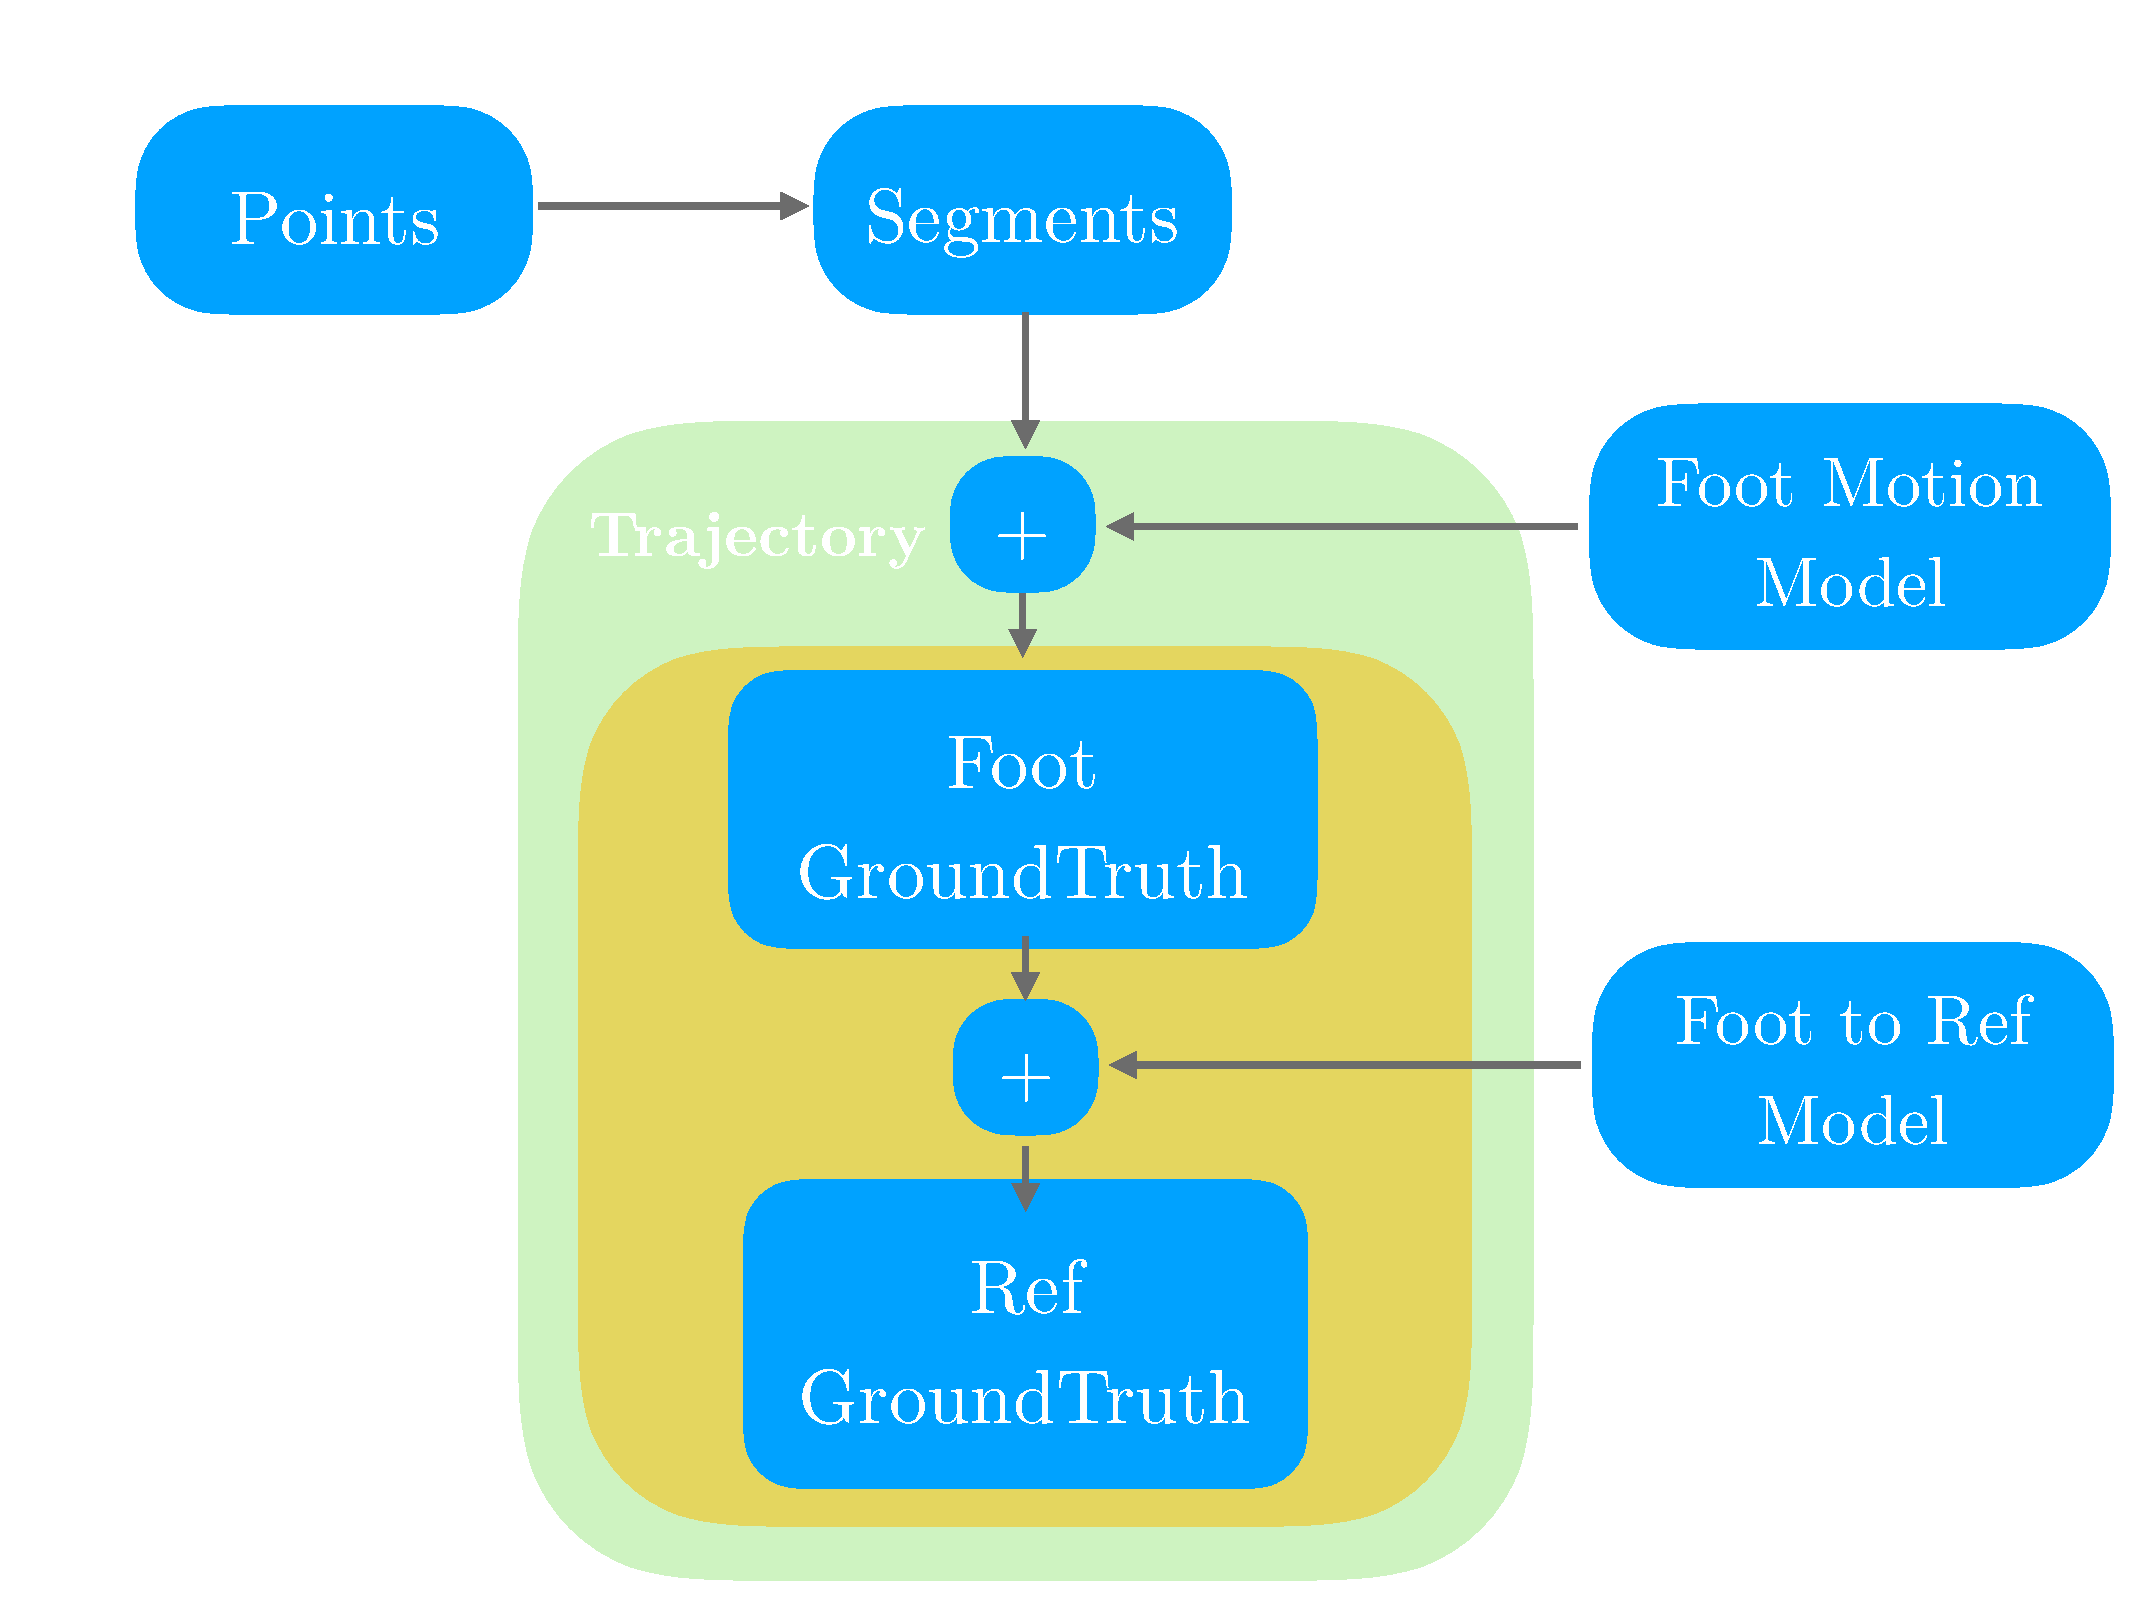
\includegraphics[width=0.8\columnwidth]{img/Design/2.pdf}
    \caption{Proceso de construcción de una trayectoria}
    \label{TrajectorySch}
    \footnotesize
    En este esquema se puede ver como el constructor de la trayectoria, genera los dos \emph{GroundTruths}, a partir de los modelos de simulación seleccionados. 
\end{figure}


%       - Explicación básica del proceso de generación de trayectorias: 
%       - Selección planta
%       - Clicks con el ratón
%       - Comprobación paredes
%       - Paso a otras plantas

El proceso de generación de trayectoria, con ayuda de la GUI, es la siguiente:

\begin{enumerate}
    \item Definimos una secuencia de puntos compatibles con la planimetría definida. Con ayuda de la GUI, podemos crear trayectorias compatibles con las restricciones la planimetría.
    \item Seleccionamos los modelos de simulación correspondientes. Existen tres tipo de modelos: modelos en un misma planta, modelos a lo largo de una escalera, y modelos a lo largo de los elevadores. Además deberemos seleccionar la función que construirá el \emph{GroundTruth} de referencia. Esta eleecciones se puede realizar con la GUI. 
    \item Por último, podemos hacer \emph{click} en el botón \emph{Generate!}
\end{enumerate}
%   - Animación 3D

\begin{figure}
    \centering
    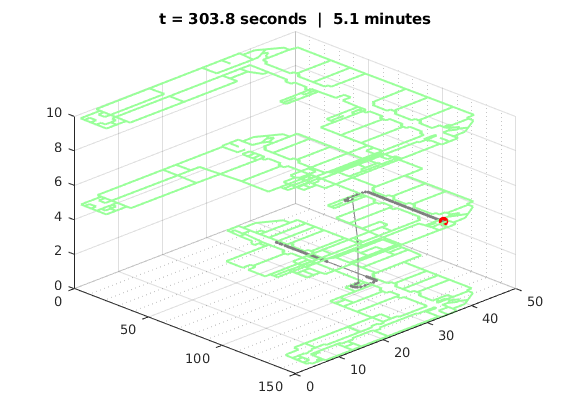
\includegraphics[width=1.0\columnwidth]{img/Design/2animation.png}
    \caption[]{Captura de una animación de una trayectoria}
    \label{fig:animation}
    \footnotesize
    La animación muestra como es la trayectoria dentro de la planimetría. El punto rojo muestra la possición de objetivo en cada instante.
\end{figure}


Al igual que el módulo de planimetría, tenemos herramientas que nos permite visualizar el resultado obtenido. El botón \emph{animate}, es capaz de mostrarnos una animación de la trayectoria dentro de  planimetría (figura \ref{fig:animation}).

% \begin{figure}[!ht]
%     \centering
%     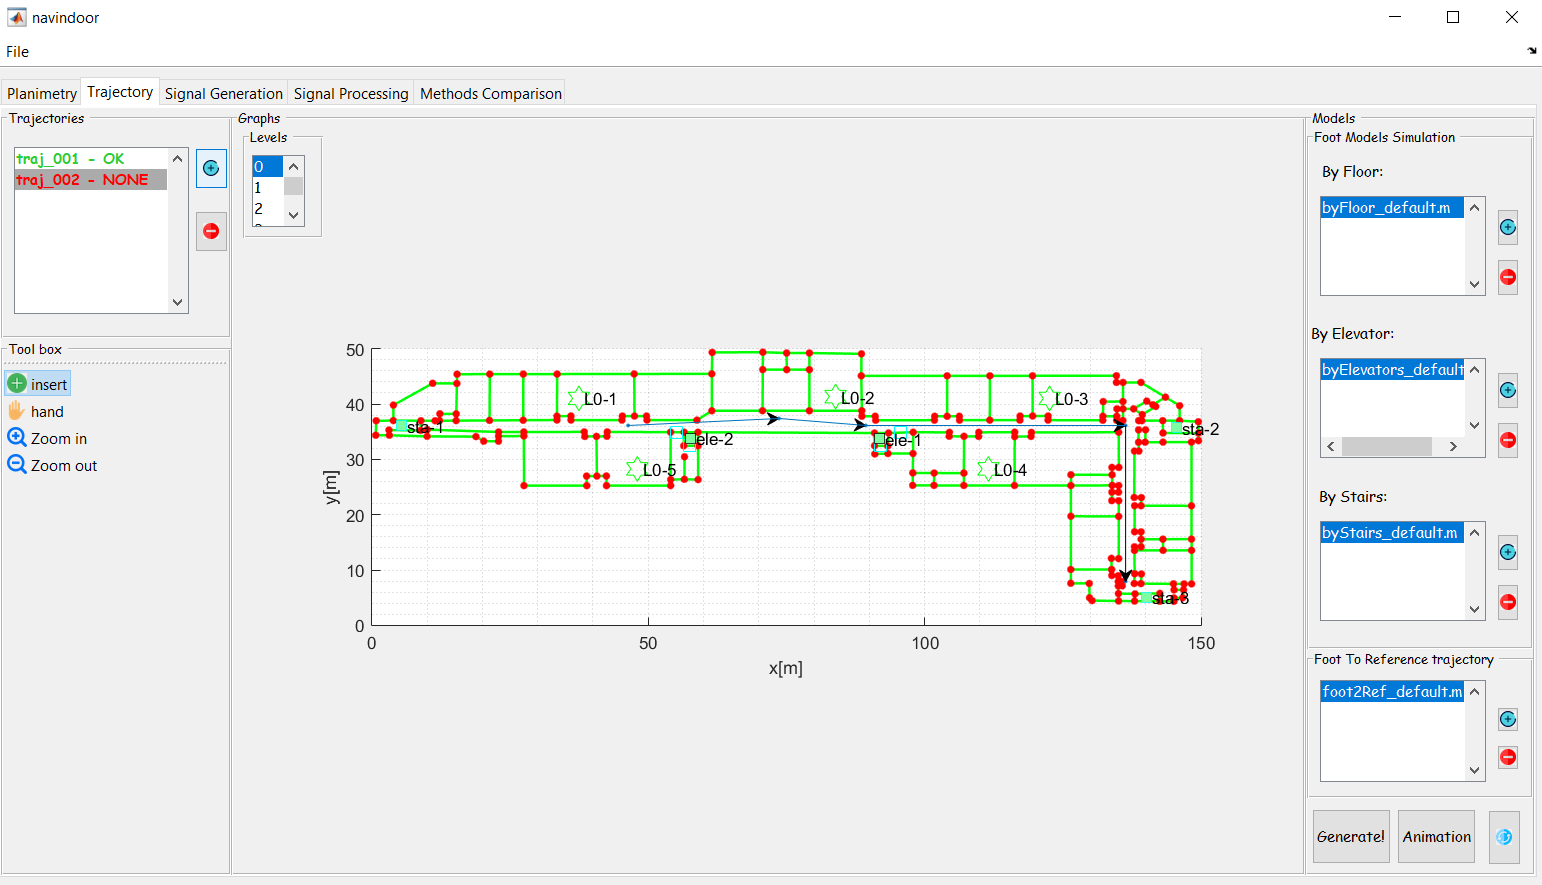
\includegraphics[width=1.5\columnwidth]{img/Design/2.PNG}
%     \caption[]{Interfaz gráfica para el diseño de las trayectorias}
%     \label{fig:interfaz2}
%     \footnotesize
%     La derecha de la imagen se encuentra los modelos de simulación. Estos son funciones de matlab, por lo que el usuario puede agregar sus propias funciones con el formato adecuado y continuar en navindoor.
% \end{figure}




% En navindoor, las trayectorias están definidas por una sucesión de puntos tridimensionales además del tiempo. De esta forma, la velocidad y aceleración de la trayectoria, puede ser extraída mediante diferenciación. Un trayectoria en navindoor, puede contender varios \emph{Ground Truth}, de la misma forma que el movimiento de un peatón puede describirse por el movimiento de distintos puntos de su cuerpo. Esto es comun cuando intentamos fusionar distintas tecnologías que no siguen extrictamente un única trayectoria.

% El proceso de generación de trayectoria es el siguiente:

% \begin{enumerate}
%     \item Definimos una secuencia de puntos compatibles con la planimetría definida
%     \item Generamos secciones entre los puntos y comprobamos por que tipo de camino transcurre el movimiento. 
%     \item Luego generamos una trayectoria del pie correspondiente a cada uno de los segmentos, teniendo en cuenta el tipo de camino. El tipo de trayectoria cambia el modelo de movimiento, ya que no es lo mismo la simulación de una persona que se mueve en una misma planta, que el movimiento cuando hay una cambio de planta.
%     \item Después, generamos una trayectoria que sea h con el movimiento del pie, pero que esta vez representara el movimiento del centro de masas.
% \end{enumerate}

% Esos pasos pueden verse representados esquemáticamente en la figura \ref{TrajectorySch}.

% Aunque para la construcción de la trayectoria es necesario un modelo de simulación del movimiento del pie, navindoor contiene modelos por defecto. Estos estan basados en el modelo propuesto en \cite{Zampella2011}. En el caso de los cambios de planta el modelo de movimiento esta simplificado a un movimiento con velocidad constante. Navindoor es capaz de modificar estos modelos como parámetros de entrada.
 
% Al igual que en el módulo de planimetría, la generación de trayectorias también contiene una interfaz gráfica que podemos ver en la figura \ref{fig:interfaz2}. Esta nos permite crear la secuencia de puntos respetando las restricciones de la planimetría, además de proporcionarnos un método simple para añadir nuevos modelos de simulación.


% \begin{figure}
%     \centering
%     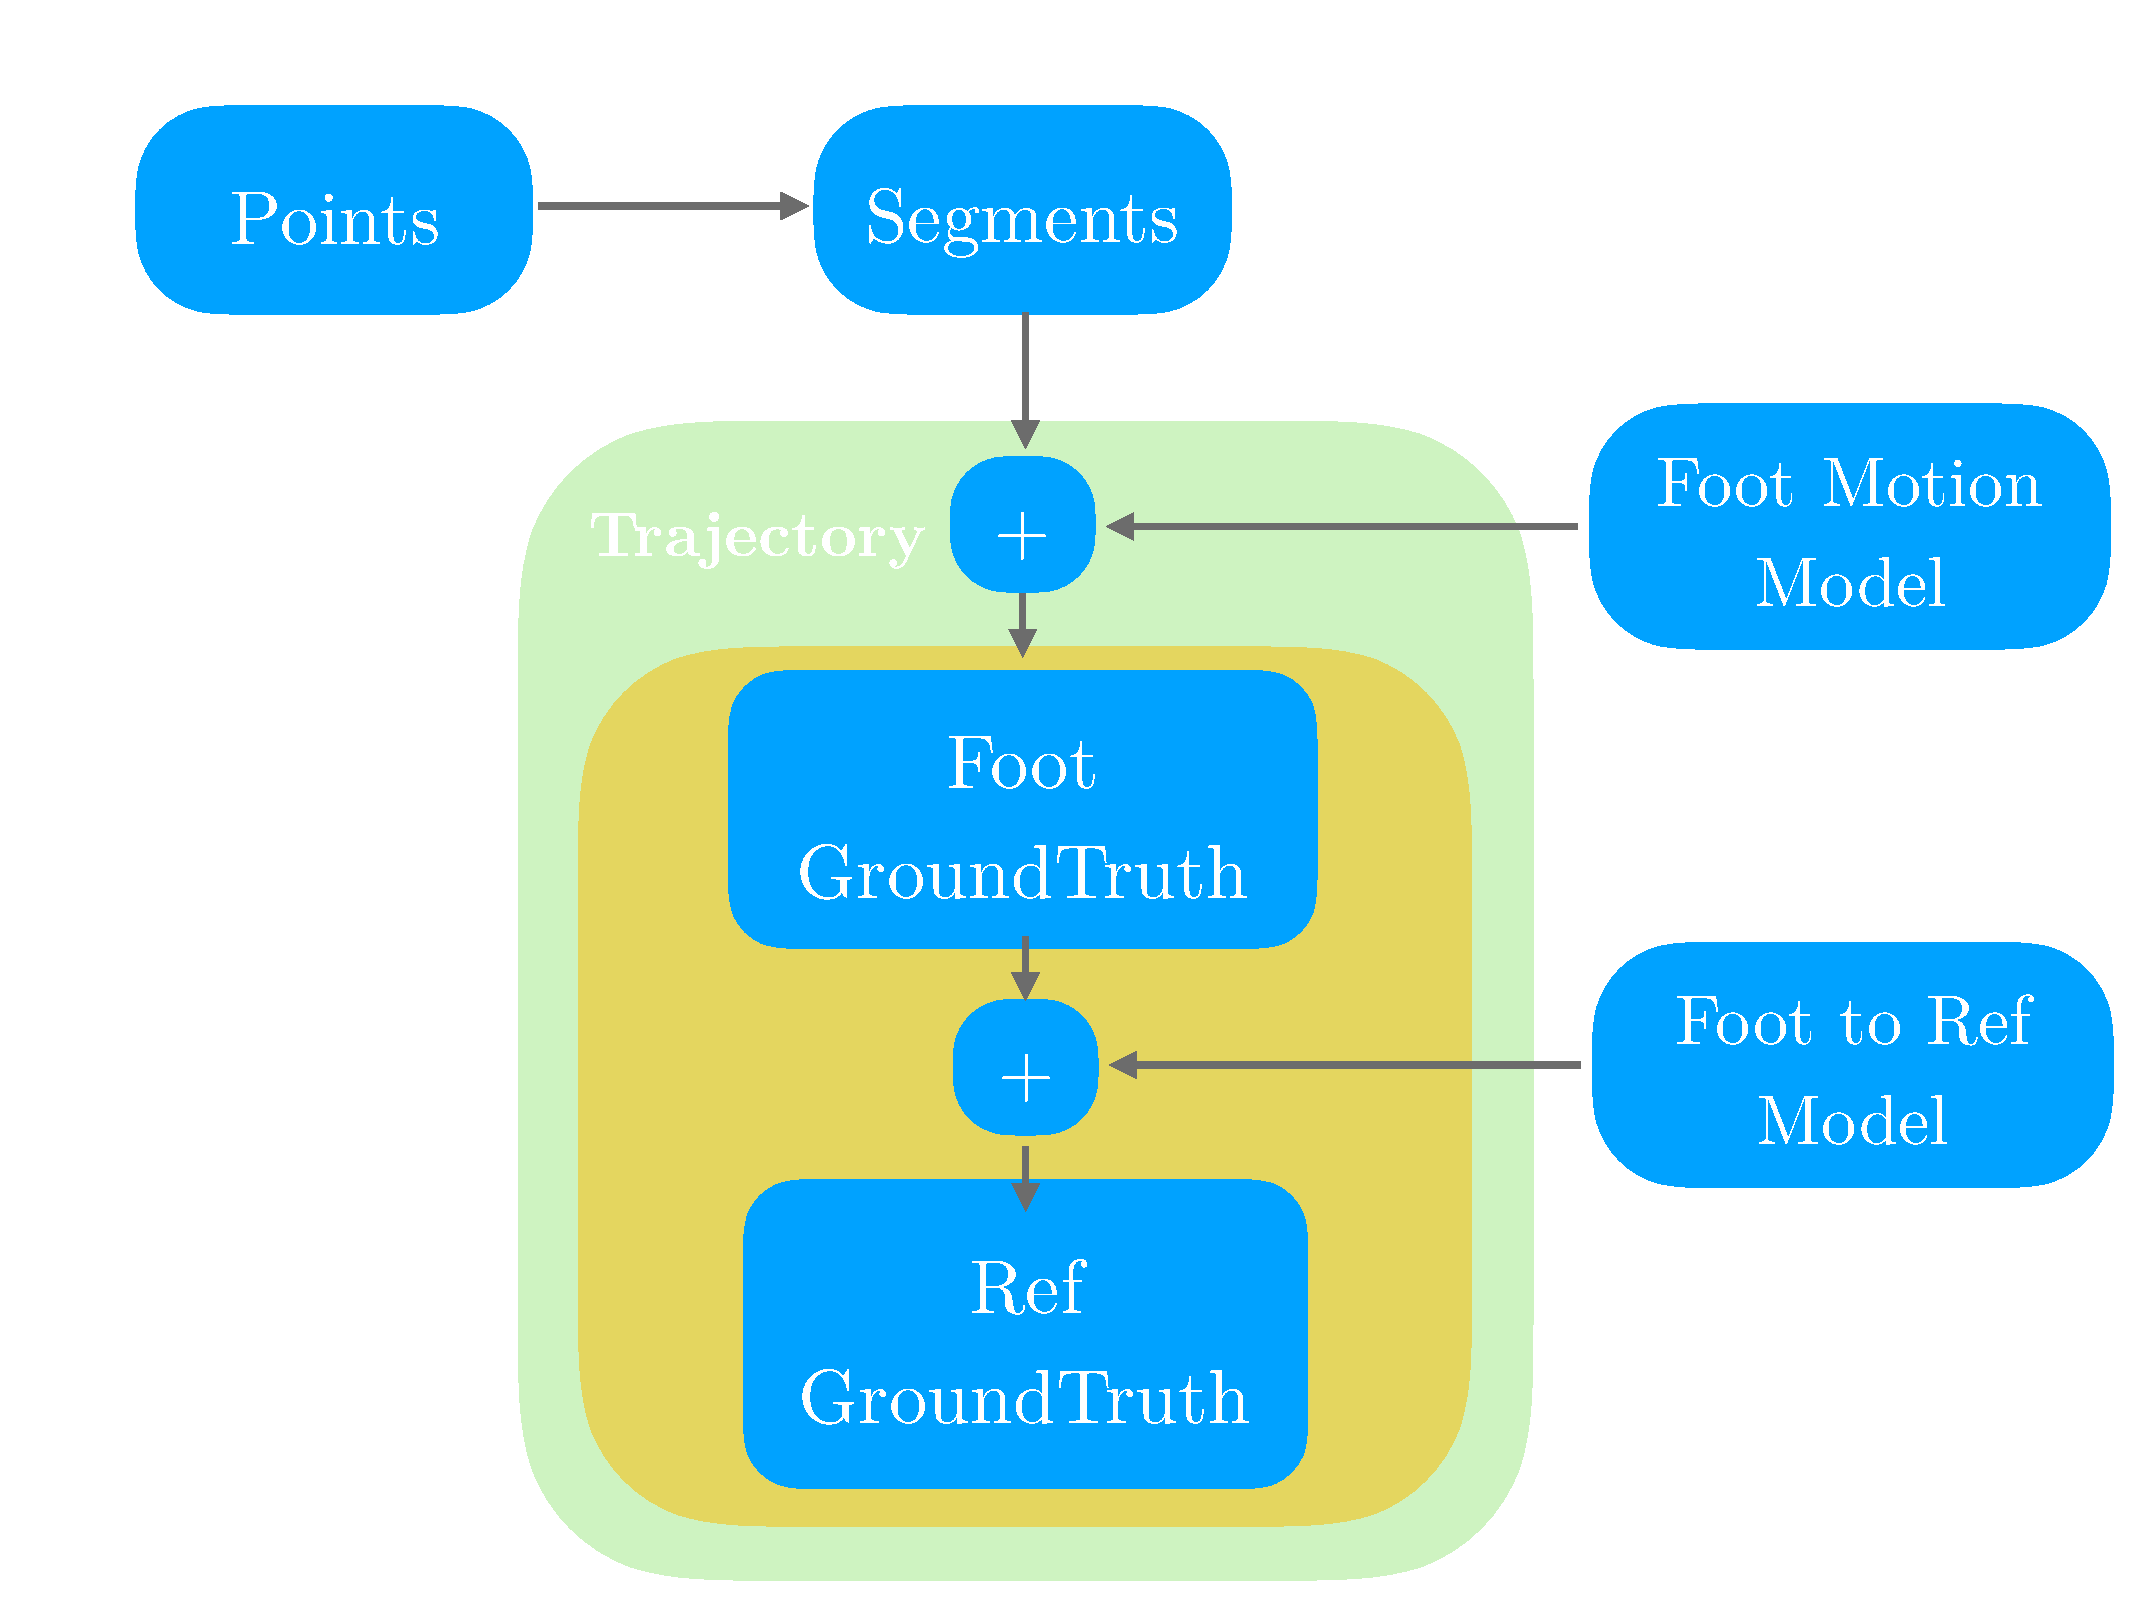
\includegraphics[width=0.8\columnwidth]{img/Design/2.pdf}
%     \caption{Proceso de construcción de una trayectoria}%
%     \label{TrajectorySch}
%     \footnotesize
%     En este esquema se puede ver como el constructor de la trayectoria, genera los dos \emph{GroundTruths}, a partir de los modelos de simulación seleccionados. 
% \end{figure}

% \begin{figure}[!ht]
%     \centering
%     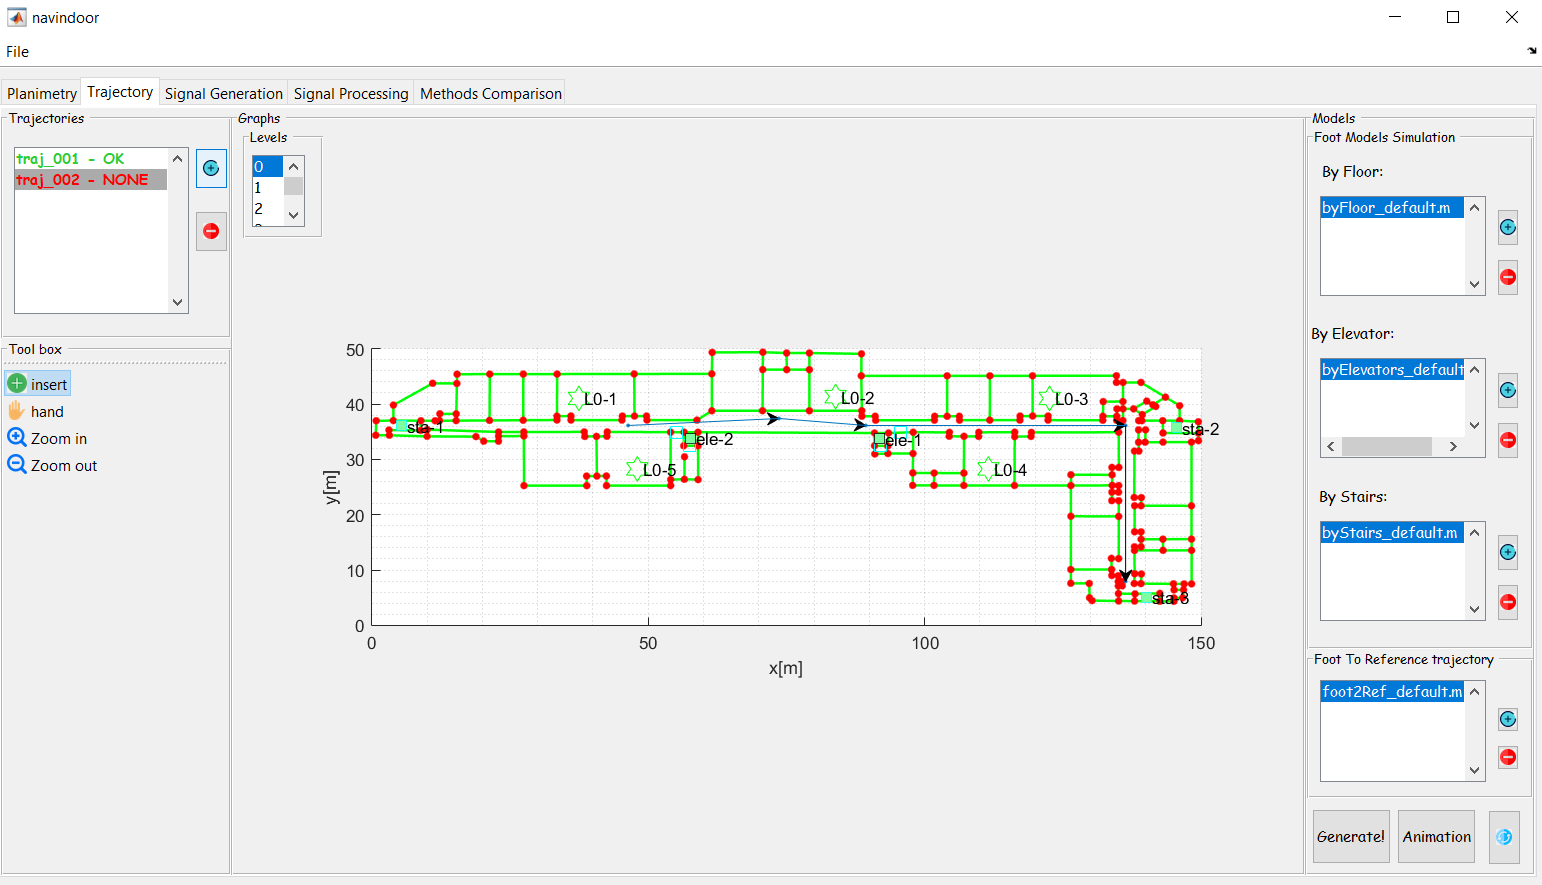
\includegraphics[width=0.8\columnwidth]{img/Design/2.PNG}
%     \caption[]{Interfaz gráfica para el diseño de las trayectorias}
%     \label{fig:interfaz2}
%     \footnotesize
%     La derecha de la imagen se encuentra los modelos de simulación. Estos son funciones de matlab, por lo que el usuario puede agregar sus propias funciones con el formato adecuado y continuar en navindoor.
% \end{figure}



